\documentclass{beamer}

\usepackage{ctex}
\usepackage{graphicx}
\usepackage{booktabs}
\usepackage{multirow}
\usepackage{tikz}
%\usetheme{AnnArbor}
\usetheme{metropolis}

\title{代数式}
\subtitle{Algebraic Expression}
\institute{Norsesun Milieu}
\author{K}
\date{\today}

\begin{document}
	\frame{\titlepage}
	%\frame{\tableofcontents}

	\section{代数式的概念}
	\subsection{课前预习}
	\begin{frame}
			在一个三角形中,若用a表示底,h表示底边上的高,则面积S=\underline{\hbox to 20mm{}}?

		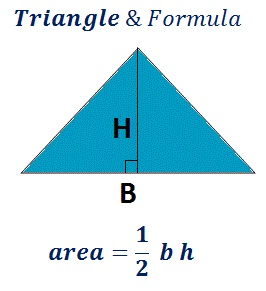
\includegraphics[width = .5\textwidth]{assets/triangle.jpg}
	\end{frame}

	\subsection{代数式定义}
	\begin{frame}
			把数与表示数的字母\ 用运算符号连接而成的式子
			\ 叫做代数式(Algebraic expression)。\ 单独一个字母或者一个数也是代					数式。例如 -5, -m。
	\end{frame}

	\section{列代数式}
	\subsection{问题}
	\begin{frame}
			x与y的和的倒数。
	\end{frame}
\end{document}